\section{Case 3C retained reactive-thermodynamic diagnosis}
\label{sec:case3c-retained-reactive-diagnosis}

\subsection*{Question}

Does the liquid \ce{CO2} fugacity produced by the retained reactive ePC-SAFT
calculation explain the decrease from the prior fugacity-only Case 3C capture,
or does the discrepancy arise primarily from another part of the coupled
transport calculation?

\subsection*{Conditions}

The absorber evaluates liquid and gas fugacity separately,
\begin{equation}
    f_{\ce{CO2}}^{L}=x_{\ce{CO2}}^{L}\phi_{\ce{CO2}}^{L}P,
    \qquad
    \Delta f_{\ce{CO2}}=f_{\ce{CO2}}^{V}-f_{\ce{CO2}}^{L},
\end{equation}
without imposing phase-equilibrium fugacity equality inside the column.  The
reactive table supplies the true liquid composition at specified liquid
temperature, pressure, and apparent composition.  The comparison uses the
2017 campaign-input Case 3C observation of \SI{89.5}{\percent} capture.

\begin{table}[htbp]
    \centering
    \caption{Fixed calculation identities and numerical checks used for the Case 3C comparison.}
    \label{tab:case3c-identities}
    \begin{threeparttable}
        \small
        \begin{tabularx}{\textwidth}{@{}>{\raggedright\arraybackslash}p{0.42\textwidth}X@{}}
            \toprule
            Quantity & Value \\
            \midrule
            Parameter-document SHA-256 & \texttt{66837ab1c9625f28...f3e133c63b} \\
            Temperature-adjustment SHA-256 & \texttt{502033bb303bd80a...e6da8} \\
            ePC-SAFT wheel SHA-256 & \texttt{81f21a6226de1fb6...615f80} \\
            Reactive liquid states & 44 evaluated; 0 failed \\
            Charge residual, maximum absolute & \num{1.25e-17} \\
            Direct/interpolated fugacity difference, maximum & \SI{1.96}{\percent} \\
            Column meshes & 21, 51, and 81 starting points \\
            \bottomrule
        \end{tabularx}
    \end{threeparttable}
\end{table}

\subsection*{Results}

The prior fugacity-only calculation predicts \SI{87.183}{\percent} capture.
The retained reactive calculation predicts \SI{71.151}{\percent} on the
51-point mesh, a difference of $-18.349$ percentage points from the
observation.  The 21-, 51-, and 81-point results span only 0.139 percentage
point, so mesh resolution does not explain the difference.

\begin{figure}[htbp]
    \centering
    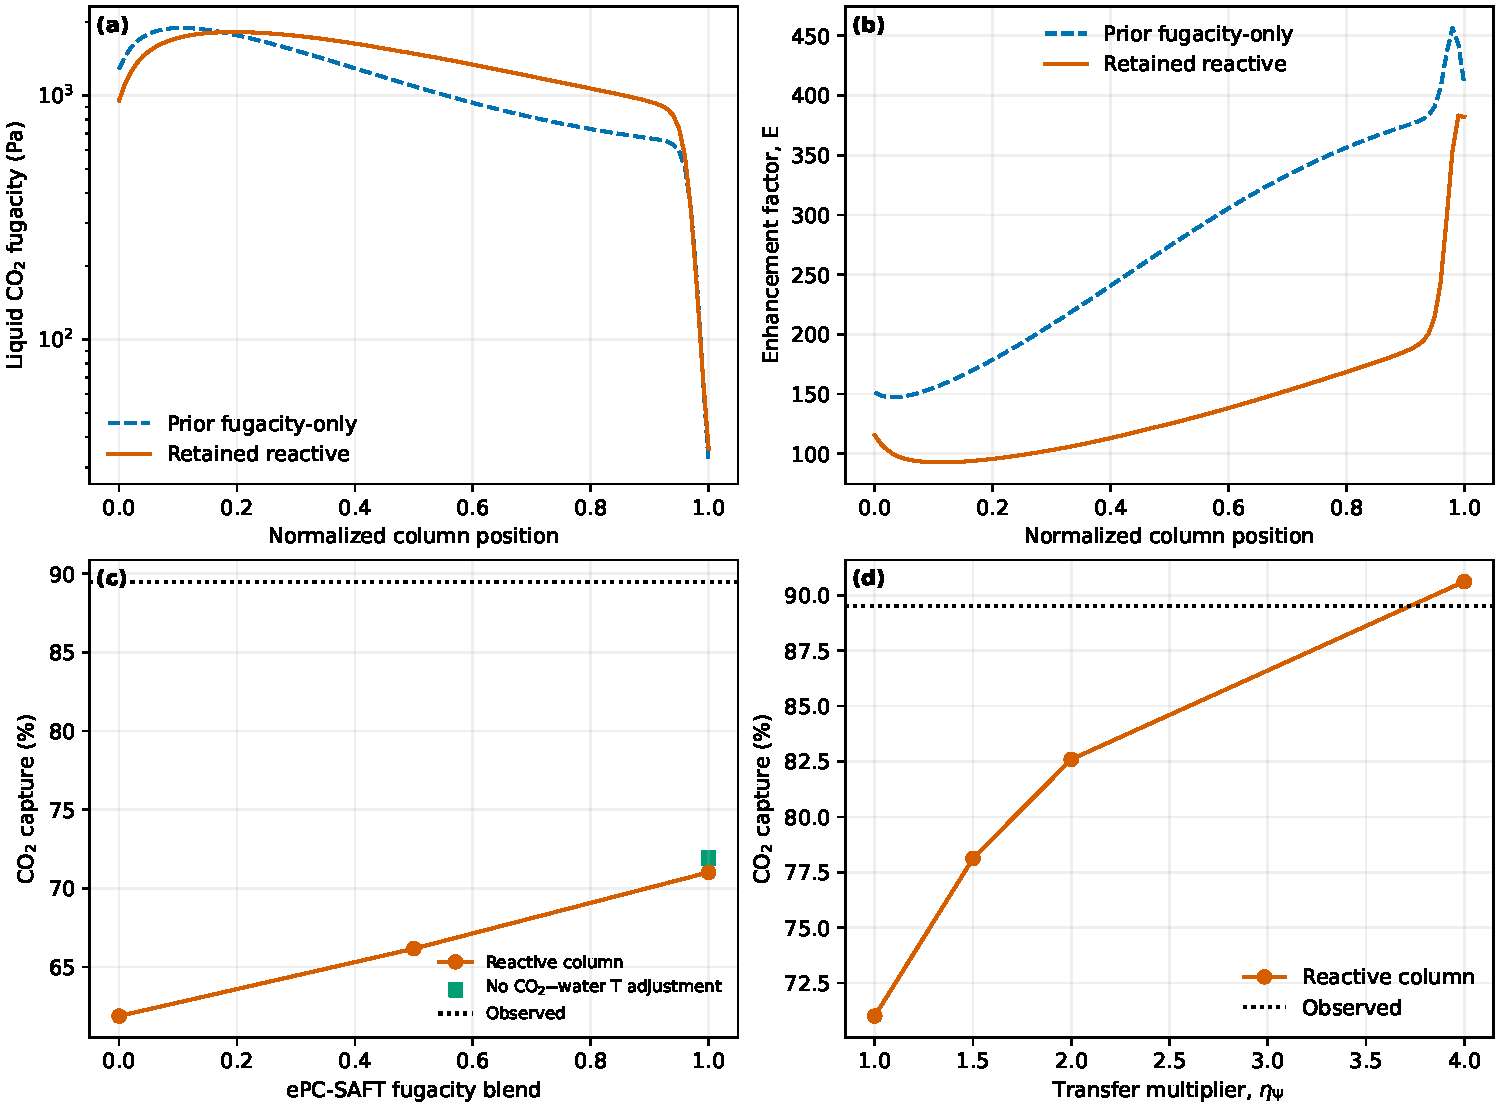
\includegraphics[width=\textwidth]{../../../../analyses/nccc_validation/results/final/figures/retained_reactive_case3c_diagnosis.pdf}
    \caption{Case 3C diagnosis from retained profile and sensitivity tables. The retained reactive calculation has moderately higher liquid \ce{CO2} fugacity than the prior fugacity-only calculation but a substantially lower enhancement factor. Replacing the ePC-SAFT fugacity closure with the Henry closure lowers capture further. Increasing the transfer multiplier can match capture only by calibrating to the same observation. Lines represent ordered model profiles or parameter sweeps; the dotted line is the measured capture.}
    \label{fig:case3c-reactive-diagnosis}
\end{figure}

On their separately converged profiles, the retained-to-prior median ratio is
1.302 for liquid \ce{CO2} fugacity, 1.543 for gas-minus-liquid fugacity driving
force, 0.483 for the enhancement factor, and 0.738 for local \ce{CO2} transfer
rate.  The liquid fugacity therefore does not decrease enough to explain the
capture loss; the driving force is larger while the transfer rate is smaller.

A controlled 21-state factorial comparison holds temperature, pressure,
apparent composition, and loading fixed.  Reactive speciation raises the
median molecular-\ce{CO2} mole fraction by a factor of 4.048.  At legacy
speciation, the retained parameters lower fugacity to 0.404 of the prior
parameter result.  With prior parameters, changing only to reactive speciation
raises fugacity by a factor of 3.888.  Applying both retained parameters and
reactive speciation gives a median fugacity ratio of 1.543 relative to the
prior-parameter, legacy-speciation calculation.  The retained parameter
changes therefore offset much of the molecular-\ce{CO2} increase rather than
amplifying it.

\begin{table}[htbp]
    \centering
    \caption{Case 3C column sensitivities. Each row changes one named calculation choice from the 21-point retained reference calculation.}
    \label{tab:case3c-sensitivities}
    \small
    \begin{tabularx}{\textwidth}{@{}>{\raggedright\arraybackslash}X S[table-format=2.2]S[table-format=+2.2]S[table-format=1.2]@{}}
        \toprule
        Calculation & {Capture (\%)} & {Error (percentage points)} & {Temperature RMSE (K)} \\
        \midrule
        Henry fugacity closure, retained speciation & 61.87 & -27.63 & 3.25 \\
        50\% Henry/ePC-SAFT fugacity blend & 66.16 & -23.34 & 3.33 \\
        Retained ePC-SAFT fugacity, $\eta_{\Psi}=1$ & 71.01 & -18.49 & 3.47 \\
        No \ce{CO2}--water temperature adjustment & 71.91 & -17.59 & 3.47 \\
        Retained ePC-SAFT fugacity, $\eta_{\Psi}=2$ & 82.59 & -6.91 & 4.20 \\
        Retained ePC-SAFT fugacity, $\eta_{\Psi}=4$ & 90.62 & +1.12 & 5.40 \\
        \bottomrule
    \end{tabularx}
\end{table}

Removing the retained \ce{CO2}--water temperature adjustment lowers liquid
fugacity by 2.2--13.7\% over the 21 controlled states and increases column
capture by only 0.90 percentage point.  Setting the retained
$k_{\ce{CO2},\mathrm{MEA}}=-0.1957$ interaction coefficient to zero while
holding reactive speciation fixed raises liquid fugacity by 32--62\%.  The
negative fitted coefficient consequently improves the transfer driving force;
it is not responsible for the low-capture result.

The explicit enhancement correlation contains molecular dissolved
\ce{CO2} in the denominator of its instantaneous enhancement limit.  The
fourfold increase in molecular \ce{CO2} therefore reduces the retained median
enhancement factor from 273.9 to 125.1.  The repository's implicit formulation
was evaluated on the same 101 profile states and gives a median overall
transfer factor 8.6\% below the explicit formulation, so it cannot close the
capture difference.

\subsection*{Interpretation}

The evidence identifies the changed molecular-\ce{CO2} partition and its use
inside the current enhancement correlation as the dominant cause of the Case
3C capture decrease.  It does not establish that the retained liquid fugacity
is accurate.  Independent pressure comparisons for the same parameter
document have structured errors of approximately a factor of two, as detailed
in \cref{sec:enhancement-pressure-consistency}.  The direct-state and mesh
tests reject interpolation and mesh resolution as material explanations for
Case 3C.  The \ce{CO2}--water temperature adjustment has a measurable but
secondary effect, and the negative \ce{CO2}--MEA interaction coefficient acts
in the direction required for higher capture.

The fourfold transfer multiplier is not independent validation: it is chosen
against the same Case 3C capture observation and worsens the temperature RMSE.
It identifies the magnitude of the transport discrepancy but is not an
acceptable predictive correction.

\clearpage
\subsection*{Manuscript admission}

\begin{table}[ht]
    \centering
    \caption{Admission assessment for possible manuscript migration.}
    \label{tab:case3c-admission}
    \small
    \begin{tabularx}{\textwidth}{@{}>{\raggedright\arraybackslash}p{0.25\textwidth}>{\raggedright\arraybackslash}p{0.17\textwidth}>{\raggedright\arraybackslash}X@{}}
        \toprule
        Proposed use & Status & Basis \\
        \midrule
        Numerical feasibility of the retained reactive liquid states & Ready & All 44 states evaluated; balance, charge, direct-state, and mesh checks passed. \\
        Explanation of the Case 3C discrepancy & Ready as a limitation or diagnostic result & Controlled comparisons identify enhancement-factor sensitivity as the dominant mechanism under the tested model. \\
        Predictive Case 3C performance claim & Not ready & Untuned capture is \SI{71.15}{\percent} versus \SI{89.5}{\percent}. \\
        Fourfold transfer correction & Reject as validation evidence & The multiplier is calibrated to Case 3C and worsens temperature agreement. \\
        General predictive absorber claim & Not ready & Only Case 3C has been tested with this retained reactive table; independent multi-case transport validation is absent. \\
        \bottomrule
    \end{tabularx}
\end{table}

\subsection*{Limitations}

This analysis covers one 30 mass-\% MEA pilot-plant case and uses interpolated
speciation from 44 retained homogeneous-liquid calculations.  The direct
checks bound interpolation error at three profile positions but do not replace
a runtime simultaneous activity/speciation solve.  The parameter perturbations
hold speciation fixed and therefore measure local fugacity sensitivity, not a
complete refit or self-consistent chemistry sensitivity.  The analysis does
not validate the enhancement correlation against independent absorber cases
and does not establish that the retained parameter set is predictive outside
its VLE and speciation comparison domain.

\FloatBarrier
